% ============================================================
% Beamer Presentation: Structure-Preserving Semigroup Learning
% 25-minute academic talk
% ============================================================
\documentclass[aspectratio=169, 11pt]{beamer}

% ---- Theme ----
\usetheme{Madrid}
\usecolortheme{whale}
\setbeamertemplate{navigation symbols}{}
\setbeamertemplate{footline}[frame number]

\newtheorem{proposition}{Proposition}

% ---- Packages ----
\usepackage{amsmath,amssymb,amsthm}
\usepackage{graphicx}
\usepackage{tikz}
\usetikzlibrary{arrows.meta, positioning, calc, patterns}
\usepackage{booktabs}
\usepackage{hyperref}

% ---- Macros ----
\newcommand{\cK}{\mathcal{K}}
\newcommand{\cE}{\mathcal{E}}
\newcommand{\cS}{\mathcal{S}}
\newcommand{\cF}{\mathcal{F}}
\newcommand{\cFN}{\mathcal{F}_N}
\newcommand{\PhiT}{\Phi_{\theta}}
\newcommand{\R}{\mathbb{R}}
\newcommand{\N}{\mathbb{N}}
\newcommand{\norm}[1]{\left\lVert #1 \right\rVert}
\newcommand{\diag}{\operatorname{diag}}
\newcommand{\softplus}{\operatorname{softplus}}
\DeclareMathOperator*{\argmin}{arg\,min}

% ---- Title ----
\title[Structure-Preserving Semigroup Learning]
{Deep Operator Learning of\\Maximum-Principle-Preserving\\Dissipative Semigroups\\for Time-Dependent PDEs}

\author[Author Name]{Author Name}
\institute{Institution}
\date{2026}

% ============================================================
\begin{document}

% ---- Title ----
\begin{frame}
\titlepage
\end{frame}

% ---- Outline ----
\begin{frame}{Outline}
\tableofcontents
\end{frame}

% ============================================================
\section{Motivation}
% ============================================================

% ---- Slide 2: The Problem ----
\begin{frame}{The Problem: Learned Operators Break Under Repetition}

\begin{columns}[T]
\begin{column}{0.55\textwidth}
\textbf{Standard operator learning} (FNO, DeepONet, ResNet):
\begin{itemize}
    \item Learn a one-step map $\hat{u}^{n+1} = \mathcal{N}_\theta(u^n)$
    \item Minimize single-step MSE
    \item \alert{No guarantee} that repeated composition stays physical
\end{itemize}

\vspace{0.3cm}
\textbf{Consequence:}
\begin{itemize}
    \item Boundary violations accumulate
    \item Energy grows instead of decaying
    \item \alert{Numerical blowup} at long times
\end{itemize}
\end{column}

\begin{column}{0.42\textwidth}
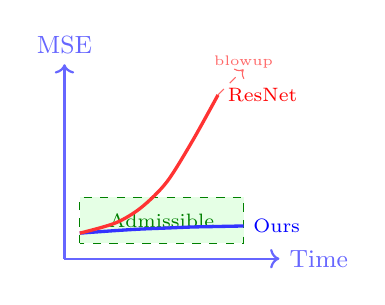
\begin{tikzpicture}[scale=0.65]
% Axes: x = Time, y = MSE
\draw[->, thick, blue!60] (0,0) -- (4.2,0) node[right]{\small Time};
\draw[->, thick, blue!60] (0,0) -- (0,3.8) node[above]{\small MSE};
% Admissible region
\fill[green!10] (0.3,0.3) rectangle (3.5,1.2);
\draw[green!50!black, dashed] (0.3,0.3) rectangle (3.5,1.2);
\node[green!50!black, font=\scriptsize] at (1.9,0.75) {Admissible};
% Latent trajectory (stays in admissible region)
\draw[very thick, blue!80, smooth] plot coordinates {(0.3,0.5) (1,0.55) (1.5,0.58) (2,0.6) (2.5,0.62) (3,0.63) (3.5,0.64)};
\node[blue, font=\scriptsize, anchor=west] at (3.5,0.64) {Ours};
% ResNet trajectory (blows up)
\draw[very thick, red!80, smooth] plot coordinates {(0.3,0.5) (1,0.7) (1.5,1.0) (2,1.5) (2.5,2.3) (3,3.2)};
\node[red, font=\scriptsize, anchor=west] at (3,3.2) {ResNet};
% Blowup indicator
\draw[red!60, ->, dashed] (3,3.2) -- (3.5,3.7);
\node[red!60, font=\tiny] at (3.5,3.85) {blowup};
\end{tikzpicture}
\end{column}
\end{columns}

\vspace{0.2cm}
\centering
\alert{Question: Can we design architectures that respect physics \emph{by construction}?}
\end{frame}

% ---- Slide 3: Structural Laws ----
\begin{frame}{Two Structural Laws of Dissipative PDEs}

\begin{exampleblock}{Running example: Fisher--KPP}
$\partial_t u = \nu\Delta u + ru(1{-}u)$ \quad with \quad $u \in [0,1]$, \quad $\cE(u) = \int_\Omega\bigl(\tfrac{\nu}{2}|\nabla u|^2 - r(\tfrac{u^2}{2}-\tfrac{u^3}{3})\bigr)\,dx \searrow$
\end{exampleblock}

\begin{columns}[T]
\begin{column}{0.48\textwidth}
\begin{block}{Maximum Principle / Invariant Region}
\[
u_0 \in \cK \;\Longrightarrow\; \cS_t u_0 \in \cK \quad \forall\, t \geq 0
\]
\begin{itemize}
    \item Fisher--KPP: $u \in [0,1]$
    \item Allen--Cahn: $u \in [-1,1]$
    \item Physical concentrations, temperatures, etc.
\end{itemize}
\end{block}
\end{column}

\begin{column}{0.48\textwidth}
\begin{block}{Energy Dissipation}
\[
\cE(\cS_t u_0) \leq \cE(u_0) \quad \forall\, t \geq 0
\]
\begin{itemize}
    \item Free energy decreases along trajectories
    \item Guarantees long-time stability
    \item Prevents spurious oscillations
\end{itemize}
\end{block}
\end{column}
\end{columns}

\vspace{0.3cm}
\centering
\textbf{Key insight:} These hold for the \emph{PDE semigroup} $(\cS_t)_{t\geq 0}$.
Can we enforce them in a \emph{learned} operator?
\end{frame}

% ---- Key Insight ----
\begin{frame}{Key Insight: Enforce Structure by Design}

\centering
\textbf{Idea:} Embed the three laws directly into the \alert{network architecture},
so they hold \emph{for every parameter}~$\theta$---no training penalty needed.

\vspace{0.4cm}
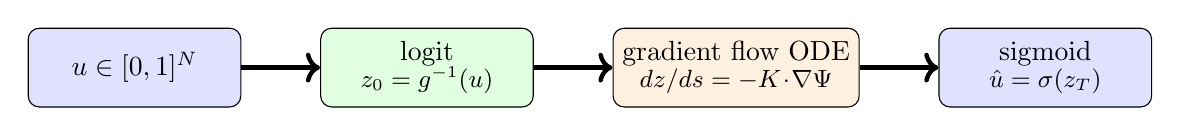
\begin{tikzpicture}[
    node distance=0.9cm,
    box/.style={draw, rounded corners, minimum height=1.0cm, minimum width=2.7cm,
                align=center, font=\normalsize},
    arr/.style={->, ultra thick}
]
% Input
\node[box, fill=blue!12] (u) {$u \in [0,1]^N$};
% Step 1
\node[box, fill=green!12, right=1.0cm of u] (z0) {logit\\[-2pt]{\small $z_0 = g^{-1}(u)$}};
% Step 2
\node[box, fill=orange!12, right=1.0cm of z0] (ode) {gradient flow ODE\\[-2pt]{\small $dz/ds = -K\!\cdot\!\nabla\Psi$}};
% Step 3
\node[box, fill=blue!12, right=1.0cm of ode] (uh) {sigmoid\\[-2pt]{\small $\hat{u} = \sigma(z_T)$}};

\draw[arr] (u) -- (z0);
\draw[arr] (z0) -- (ode);
\draw[arr] (ode) -- (uh);
\end{tikzpicture}

\vspace{0.5cm}
\begin{columns}[T]
\begin{column}{0.3\textwidth}
\centering
\textcolor{green!50!black}{\textbf{$g=\sigma$}}\\[3pt]
{\small Bounded output}\\[2pt]
$\Rightarrow$ admissibility
\end{column}
\begin{column}{0.35\textwidth}
\centering
\textcolor{orange!70!black}{\textbf{$K \succ 0$ + gradient flow}}\\[3pt]
{\small Energy decreases}\\[2pt]
$\Rightarrow$ dissipation
\end{column}
\begin{column}{0.3\textwidth}
\centering
\textcolor{blue!70!black}{\textbf{ODE flow}}\\[3pt]
{\small Unique trajectories}\\[2pt]
$\Rightarrow$ semigroup
\end{column}
\end{columns}
\end{frame}

% ---- Why Standard Networks Fail ----
\begin{frame}{Why Standard Networks Fail at Long Times}

\begin{columns}[T]
\begin{column}{0.48\textwidth}
\textbf{ResNet / FNO trained for one step:}
\begin{itemize}
    \item Minimize $\|\mathcal{N}_\theta(u^n) - u^{n+1}\|^2$
    \item No structural constraint
    \item Single-step error is small
\end{itemize}

\vspace{0.2cm}
\textbf{But repeated composition:}
\begin{itemize}
    \item $\varepsilon_{\mathrm{sg}} > 0$ $\Rightarrow$ errors \alert{accumulate}
    \item Boundary violations $\to$ unphysical states
    \item Energy grows $\to$ spurious oscillations
    \item Eventually: \alert{numerical blowup}
\end{itemize}
\end{column}

\begin{column}{0.5\textwidth}
\begin{exampleblock}{Fisher--KPP at $T=20$}
\begin{center}
\small
\renewcommand{\arraystretch}{1.15}
\begin{tabular}{lcc}
\toprule
Method & BV & Energy \\
\midrule
FNO & $15.4\%$ & grows \\
ResNet & blowup & blowup \\
\textbf{Ours} & $\mathbf{0.00}$ & $\mathbf{100\%}$ \\
\bottomrule
\end{tabular}
\end{center}
\end{exampleblock}

\vspace{0.15cm}
\begin{alertblock}{Root cause}
$\varepsilon_{\mathrm{sg}} > 0$ in standard networks:\\
\centering $\Phi(\Phi(u,\tau_1),\tau_2) \neq \Phi(u,\tau_1{+}\tau_2)$
\end{alertblock}
\end{column}
\end{columns}
\end{frame}

% ============================================================
\section{Semigroup Formulation}
% ============================================================

% ---- Slide 4: Definition ----
\begin{frame}{Structure-Preserving Deep Semigroup Learner}

\begin{definition}[Target specification]
A learned evolution family $\PhiT(\cdot,\tau):\cK\to\cK$ is \textbf{structure-preserving} if:
\begin{align}
    \text{(S1)}\quad & \PhiT(u,0) = u & \text{(identity)} \\
    \text{(S2)}\quad & \PhiT(u,\tau) \in \cK & \text{(admissibility)} \\
    \text{(S3)}\quad & \PhiT(\PhiT(u,\tau_1),\tau_2) = \PhiT(u,\tau_1{+}\tau_2) & \text{(semigroup)} \\
    \text{(S4)}\quad & \cE(\PhiT(u,\tau)) \leq \cE(u) & \text{(dissipation)}
\end{align}
\end{definition}

\vspace{0.2cm}
\begin{itemize}
    \item (S1)--(S3) define an \emph{evolution family} for repeated composition
    \item (S4) ensures energy stability
    \item These are \alert{architecture-level} guarantees: hold for \emph{every} $\theta$
\end{itemize}
\end{frame}

% ---- Slide 5: Error Decomposition ----
\begin{frame}{Error Propagation Under Repeated Composition}

\begin{theorem}[Error decomposition]
\[
\norm{u^n - \cS_{n\Delta t} u_0}
\;\leq\;
\underbrace{\varepsilon_{\mathrm{app}}}_{\text{approximation}}
\;+\;
n \cdot \underbrace{\varepsilon_{\mathrm{sg}}}_{\text{semigroup defect}}
\]
where
\begin{itemize}
    \item $\varepsilon_{\mathrm{app}}$: trajectory-level fit from $u_0$
    \item $\varepsilon_{\mathrm{sg}} = \sup_u \norm{\PhiT(\PhiT(u,\tau_1),\tau_2) - \PhiT(u,\tau_1{+}\tau_2)}$
\end{itemize}
\end{theorem}

\vspace{0.2cm}
\begin{alertblock}{Why this matters}
If $\varepsilon_{\mathrm{sg}} > 0$ (generic neural network), errors \textbf{accumulate linearly} in $n$.
If $\varepsilon_{\mathrm{sg}} = 0$ (exact semigroup), only approximation error remains.
\end{alertblock}
\end{frame}

% ============================================================
\section{Latent Architecture}
% ============================================================

% ---- Architecture Definition ----
\begin{frame}{Network Structure: Latent Dissipative Flow}

\small
\textbf{Step 1. Bounded latent map.} Let $\sigma(\xi) = (1+e^{-\xi})^{-1}$.
Define $g:\R^N \to (m,M)^N$ componentwise by
\[
g(z)_i = m + (M{-}m)\,\sigma(z_i), \qquad
g^{-1}(u)_i = \log\!\Bigl(\frac{u_i - m}{M - u_i}\Bigr).
\]
\begin{itemize}
    \item $\sigma: \R \to (0,1)$ is $C^\infty$, strictly increasing
    \item $g$ maps \emph{all} of $\R^N$ into $(m,M)^N$ $\Rightarrow$ \textcolor{green!50!black}{admissibility by construction}
\end{itemize}

\vspace{0.3cm}
\textbf{Step 2. Latent energy (reaction--diffusion ansatz).}
\[
\Psi_\theta(z) = \sum_{i=1}^N V_\theta(z_i) + \frac{1}{2}\sum_{i,j=1}^N a_{ij}^{(\theta)}(z_i - z_j)^2
\]
\begin{itemize}
    \item $V_\theta \in C^1(\R;\R)$: scalar potential (MLP + $\frac{\beta_V}{2}\xi^2$, $\rho=$ softplus)
    \item $a_{ij}^{(\theta)} = m_{ij}\,\mathrm{softplus}(e_i^\top e_j) \geq 0$: learned interaction ($m_{ij}$: local mask, $e_i \in \R^{r_A}$: embeddings)
\end{itemize}
\end{frame}

\begin{frame}{Network Structure: Latent Dissipative Flow (cont.)}

\small
\textbf{Step 3. Diagonal PSD mobility.}
\[
K_\theta(z) = \mathrm{diag}\bigl(k_{\theta,1}(z),\dots,k_{\theta,N}(z)\bigr), \qquad
k_{\theta,i}(z) = \mathrm{softplus}\bigl(\mathrm{StencilMLP}(z_{\mathcal{N}(i)})\bigr) > 0
\]
\begin{itemize}
    \item StencilMLP: local input $z_{\mathcal{N}(i)}$ (periodic padding), MLP + softplus
    \item $K_\theta \succ 0$ pointwise $\Rightarrow$ \textcolor{orange!70!black}{dissipation by construction}
\end{itemize}

\vspace{0.3cm}
\textbf{Step 4. Latent gradient-flow ODE.}
\[
\partial_s z_i = -k_{\theta,i}(z)\!\left(V_\theta'(z_i) + 2\textstyle\sum_j a_{ij}^{(\theta)}(z_i - z_j)\right), \qquad z(0) = g^{-1}(u)
\]
\begin{itemize}
    \item $dz/ds = -K_\theta(z)\,\nabla\Psi_\theta(z)$: gradient flow in latent space
    \item Integrated by RK4 with $M=30$ substeps per $\tau$
\end{itemize}

\vspace{0.3cm}
\textbf{Step 5. One-step operator.}
\[
\PhiT(u,\tau) := g\bigl(\varphi_\theta^\tau(g^{-1}(u))\bigr), \qquad \varphi_\theta^\tau = \text{ODE flow for time } \tau
\]

\vspace{0.15cm}
\centering
{\color{gray} Each component is chosen to enforce one structural guarantee:}
$\sigma$ \textcolor{green!50!black}{$\to$ admissible},
\;$K_\theta\succ 0$ \textcolor{orange!70!black}{$\to$ dissipative},
\;flow \textcolor{blue!70!black}{$\to$ semigroup}.
\end{frame}


% ---- Network Architecture (full diagram) ----
\begin{frame}{Network Architecture}

\centering
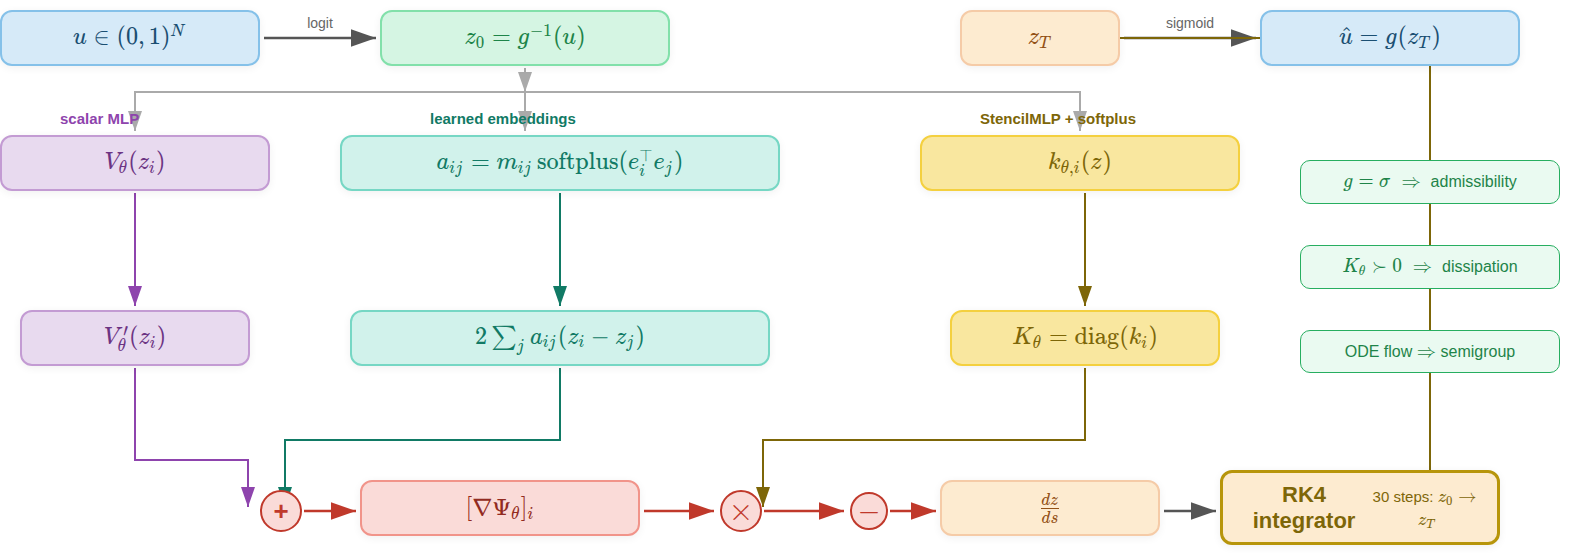
\includegraphics[width=\textwidth, height=0.9\textheight, keepaspectratio]{architecture_diagram.png}
\end{frame}

% ---- Slide 7: Three Guarantees ----
\begin{frame}{Three Guarantees by Construction}

\begin{columns}[T]
\begin{column}{0.32\textwidth}
\begin{alertblock}{Admissibility}
$u = \sigma(z) \in (0,1)^N$

\vspace{0.15cm}
\centering
\Large $\checkmark$\\[2pt]
\normalsize Holds for \emph{all} $z \in \R^N$
\end{alertblock}
\end{column}

\begin{column}{0.32\textwidth}
\begin{alertblock}{Dissipation}
$\frac{d\Psi}{ds} = -K\norm{\nabla\Psi}^2 \leq 0$

\vspace{0.15cm}
\centering
\Large $\checkmark$\\[2pt]
\normalsize $K \succ 0$ by design
\end{alertblock}
\end{column}

\begin{column}{0.32\textwidth}
\begin{alertblock}{Semigroup}
$\PhiT \circ \PhiT = \PhiT$

\vspace{0.15cm}
\centering
\Large $\checkmark$\\[2pt]
\normalsize ODE flow uniqueness
\end{alertblock}
\end{column}
\end{columns}

\vspace{0.4cm}
\centering
\textbf{All three hold for \emph{every} parameter $\theta$, independent of training.}
\end{frame}

% ---- Slide 8: Neural Parametrization ----
\begin{frame}{Neural Parametrization}

\begin{columns}[T]
\begin{column}{0.48\textwidth}
\begin{block}{Scalar potential $V_\theta$}
\[
V_\theta(z_i) = \mathrm{MLP}(z_i) + \tfrac{\beta}{2} z_i^2
\]
\begin{itemize}
    \item softplus activation ($C^\infty$)
    \item $\beta \geq 0$: quadratic growth for coercivity
\end{itemize}
\end{block}

\begin{block}{Interaction coefficients}
\[
a_{ij} = m_{ij}\,\softplus(e_i^\top e_j) \geq 0
\]
\begin{itemize}
    \item $m_{ij}$: local interaction mask ($|i{-}j| \leq r$)
    \item $e_i \in \R^8$: learned embeddings
\end{itemize}
\end{block}
\end{column}

\begin{column}{0.48\textwidth}
\begin{block}{Mobility $K_\theta$}
\[
k_{\theta,i}(z) = \mathrm{StencilMLP}(z_{\mathcal{N}(i)}) + \epsilon
\]
\begin{itemize}
    \item Local stencil input (periodic padding)
    \item $\softplus + \epsilon > 0$: positive diagonal
\end{itemize}
\end{block}
\end{column}
\end{columns}
\end{frame}

% ---- Training Loss ----
\begin{frame}{Training Loss}

\centering
\begin{block}{Training objective}
\[
\mathcal{L} = \mathcal{L}_{\mathrm{step}} = \|\Phi_\theta(u,\tau) - u^{\mathrm{ref}}\|^2
\]
\end{block}

\vspace{0.5cm}
\begin{columns}[T]
\begin{column}{0.48\textwidth}
\begin{exampleblock}{What we optimize}
\begin{itemize}
    \item One-step prediction: match PDE snapshot at $t+\tau$
    \item Standard MSE loss
    \item No auxiliary regularization terms
\end{itemize}
\end{exampleblock}
\end{column}

\begin{column}{0.48\textwidth}
\begin{exampleblock}{Why no other losses?}
\begin{itemize}
    \item \textbf{Semigroup:} enforced by ODE flow uniqueness; RK4 truncation $\sim 10^{-14}$ is negligible
    \item \textbf{Dissipation:} enforced by $K_\theta \succ 0$ + gradient flow ($d\Psi/ds \leq 0$)
    \item \textbf{Both verified as post-training diagnostics}
\end{itemize}
\end{exampleblock}
\end{column}
\end{columns}
\end{frame}

% ============================================================
\section{Theoretical Results}
% ============================================================

% ---- Slide 9: Transfer Theorem ----
\begin{frame}{Transfer Theorem}

\begin{theorem}[Continuous $\to$ discrete $\to$ latent]
Under Assumptions 1--3, for initial data $u_0 \in \cK$:
\[
\norm{\PhiT(u_0^N, n\Delta t) - \cS_{n\Delta t} u_0}
\;\leq\;
C(N) + n\Delta t\,\varepsilon_{\mathrm{match}}
\]
where
\begin{itemize}
    \item $C(N)$: spatial discretization rate (Proposition 8)
    \item $\varepsilon_{\mathrm{match}}$: generator matching error
\end{itemize}
\end{theorem}

\vspace{0.2cm}
\begin{itemize}
    \item Decomposes the chain: PDE $\to$ semidiscrete $\to$ latent architecture
    \item $C(N) \to 0$ as $N \to \infty$ (consistent spatial discretization)
    \item $\varepsilon_{\mathrm{match}} \to 0$: universal approximation of the generator
\end{itemize}
\end{frame}

% ---- Slide 10: Universal Approximation ----
\begin{frame}{Expressivity: Universal Approximation}

\begin{proposition}[Gradient-type generators]
For any smooth semidiscrete generator $\cFN$ of reaction--diffusion type, the latent architecture can approximate $\cFN$ to arbitrary accuracy on compact subsets of $(m,M)^N$.
\end{proposition}

\vspace{0.2cm}
\textbf{Proof structure (4 steps):}
\begin{enumerate}
    \item MLP approximation of scalar potential $V$
    \item Embedding approximation of interaction coefficients $a_{ij}$
    \item Stencil MLP approximation of mobility $K$
    \item Product composition with Lipschitz stability
\end{enumerate}

\vspace{0.2cm}
\begin{block}{Scope}
\begin{itemize}
    \item \textbf{Applies to:} Fisher--KPP, Allen--Cahn (gradient-type generators)
    \item \textbf{Does not formally apply to:} Burgers (skew-symmetric convective term)
    \item Good empirical results for Burgers suggest expressivity beyond gradient class
\end{itemize}
\end{block}
\end{frame}

% ---- Slide 11: Architectural Guarantees Summary ----
\begin{frame}{Summary: What is Proved vs.\ What is Open}

\begin{center}
\begin{tabular}{lcc}
\toprule
\textbf{Property} & \textbf{Level} & \textbf{Status} \\
\midrule
Admissibility $u \in (0,1)^N$ & Architecture & \textcolor{green!60!black}{\textbf{Exact}} \\
Energy dissipation & Architecture & \textcolor{green!60!black}{\textbf{Exact}} \\
Semigroup composition & Architecture & \textcolor{green!60!black}{\textbf{Exact}} \\
Spatial convergence $C(N) \to 0$ & Semidiscrete & \textcolor{green!60!black}{\textbf{Proved}} \\
Generator approximation & Latent & \textcolor{green!60!black}{\textbf{Proved}} \\
Global flow existence ($\beta_V = 0$) & Architecture & \textcolor{orange}{\textbf{Open}} \\
PDE-level transfer & Full chain & \textcolor{orange}{\textbf{Open}} \\
\bottomrule
\end{tabular}
\end{center}

\vspace{0.2cm}
\centering
\textbf{Architecture-level guarantees are unconditional.}
Transfer to PDE level is formulated as open problems.
\end{frame}

% ============================================================
\section{Numerical Experiments}
% ============================================================

% ---- Slide 12: Setup ----
\begin{frame}{Experimental Setup}

\begin{columns}[T]
\begin{column}{0.48\textwidth}
\begin{block}{Three PDE Benchmarks}
\begin{enumerate}
    \item \textbf{Fisher--KPP}: $\partial_t u = \nu\Delta u + ru(1{-}u)$, $\;u \in [0,1]$
    \item \textbf{Allen--Cahn}: $\partial_t u = \varepsilon\Delta u + u - u^3$, $\;u \in [-1,1]$
    \item \textbf{Burgers}: $\partial_t u = \nu\partial_{xx}u - u\partial_x u$, $\;u \in [-1,1]$
\end{enumerate}
\end{block}
\end{column}

\begin{column}{0.48\textwidth}
\begin{block}{Configuration}
\begin{itemize}
    \item $N = 64$ spatial nodes, periodic BC\\[2pt]\textcolor{blue!70}{\scriptsize (2D extension: $32\times32$, in progress)}
    \item 1000 training / 50 validation trajectories
    \item RK4 with $M = 30$ substeps per $\tau$
    \item AdamW, lr$=10^{-3}$, cosine decay
\end{itemize}
\end{block}

\begin{block}{Baselines}
\begin{itemize}
    \item \textbf{ResNet}: 4-block residual network (41.6K params)
    \item \textbf{FNO}: 4-layer Fourier Neural Operator (17.5K params)
    \item \textbf{Ours}: Latent semigroup (9.6K params)
\end{itemize}
\end{block}
\end{column}
\end{columns}
\end{frame}

% ---- Slide 13: Fisher-KPP Results ----
\begin{frame}{Fisher--KPP: Short-Time Comparison ($T = 2$)}

\begin{columns}[T]
\begin{column}{0.52\textwidth}
\centering
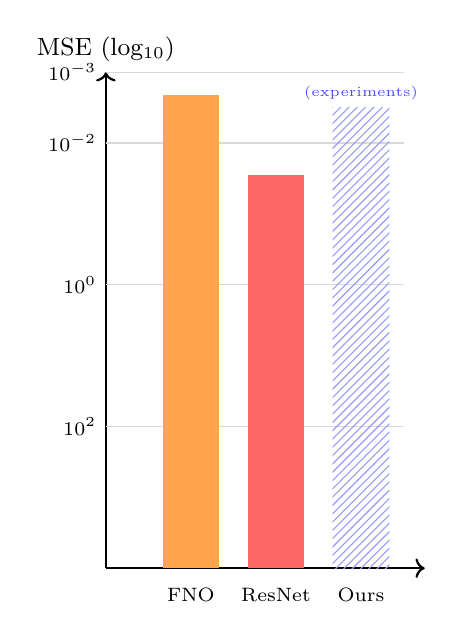
\begin{tikzpicture}[scale=0.9]
% Bar chart: Rollout MSE (log scale)
\draw[->, thick] (0,0) -- (0,7) node[above, font=\small]{MSE (log$_{10}$)};
\draw[->, thick] (0,0) -- (4.5,0);
% Grid lines
\foreach \y/\lbl in {7/$10^{-3}$, 6/$10^{-2}$, 4/$10^{0}$, 2/$10^{2}$} {
    \draw[gray!30] (0, \y) -- (4.2, \y);
    \node[left, font=\scriptsize] at (0, \y) {\lbl};
}
% FNO bar
\fill[orange!70] (0.8,0) rectangle (1.6, {-log10(2.10e-3)+4});
\node[below, font=\scriptsize] at (1.2, -0.15) {FNO};
% ResNet bar
\fill[red!60] (2.0,0) rectangle (2.8, {-log10(2.86e-2)+4});
\node[below, font=\scriptsize] at (2.4, -0.15) {ResNet};
% Latent bar (placeholder - dashed)
\fill[blue!60, pattern=north east lines, pattern color=blue!40] (3.2,0) rectangle (4.0, 6.5);
\node[below, font=\scriptsize] at (3.6, -0.15) {Ours};
\node[font=\tiny, blue!70] at (3.6, 6.7) {(experiments)};
\end{tikzpicture}
\end{column}

\begin{column}{0.45\textwidth}
\small
\textbf{Key guarantees (by construction):}

\vspace{0.2cm}
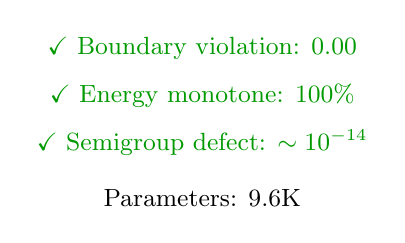
\begin{tikzpicture}[
    check/.style={green!60!black, font=\small},
    cross/.style={red!60, font=\small}
]
\node[check] at (0, 2.0) {$\checkmark$ Boundary violation: $0.00$};
\node[check] at (0, 1.4) {$\checkmark$ Energy monotone: $100\%$};
\node[check] at (0, 0.8) {$\checkmark$ Semigroup defect: $\sim 10^{-14}$};
\node at (0, 0.1) {\small Parameters: 9.6K};
\end{tikzpicture}

\vspace{0.3cm}
\textbf{vs.\ baselines:}
\begin{itemize}
    \item FNO: BV $4.6\times10^{-4}$, defect $2.2\times10^{-5}$
    \item ResNet: BV $7.2\times10^{-4}$, defect $2.1\times10^{-4}$
\end{itemize}
\end{column}
\end{columns}
\end{frame}

% ---- Slide 14: Long-time Rollout ----
\begin{frame}{Long-Time Rollout: Why Structure Matters}

\begin{columns}[T]
\begin{column}{0.55\textwidth}
\centering
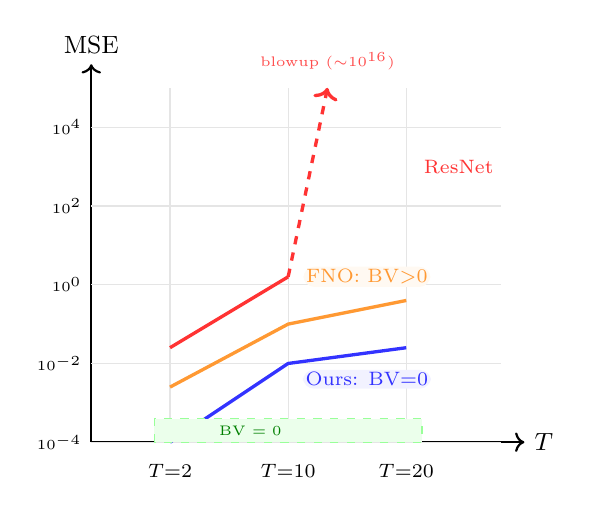
\begin{tikzpicture}[scale=1.0]
% Axes — using log-compressed y: y = 0.5*(log10(MSE)+4)
\draw[->, thick] (0,0) -- (5.5,0) node[right, font=\small]{$T$};
\draw[->, thick] (0,0) -- (0,4.8) node[above, font=\small]{MSE};
% Grid — log-spaced labels
\foreach \y/\lbl in {0/$10^{-4}$, 1/$10^{-2}$, 2/$10^{0}$, 3/$10^{2}$, 4/$10^{4}$} {
    \draw[gray!20] (0,\y) -- (5.2,\y);
    \node[left, font=\tiny] at (0,\y) {\lbl};
}
\foreach \x/\lbl in {1/$T{=}2$, 2.5/$T{=}10$, 4/$T{=}20$} {
    \draw[gray!20] (\x,0) -- (\x,4.5);
    \node[below, font=\scriptsize] at (\x,-0.15) {\lbl};
}
% Latent line: MSE ~ 1e-4 at T=2, ~4e-1 at T=10, ~4e-1 at T=20
% y = 0.5*(log10(MSE)+4): 1e-4->0, 4e-1->1.7
\draw[very thick, blue!80] (1, 0.0) -- (2.5, 1.0) -- (4, 1.2);
\node[blue!80, font=\scriptsize, fill=blue!5, rounded corners, inner sep=1pt] at (3.5, 0.8) {Ours: BV=0};
\draw[very thick, orange!80] (1, 0.7) -- (2.5, 1.5) -- (4, 1.8);
\node[orange!80, font=\scriptsize, fill=orange!5, rounded corners, inner sep=1pt] at (3.5, 2.1) {FNO: BV$>$0};
% ResNet: 2.9e-2 at T=2, 1.6 at T=10, ~10^16 at T=20
% y: -1.54->1.23, 0.2->2.1, 16->10 (off chart)
\draw[very thick, red!80] (1, 1.2) -- (2.5, 2.1);
\draw[very thick, red!80, ->, dashed] (2.5, 2.1) -- (3.0, 4.5);
\node[red!70, font=\tiny, anchor=south] at (3.0, 4.6) {blowup (${\sim}10^{16}$)};
\node[right, font=\scriptsize, red!80] at (4.1, 3.5) {ResNet};
% Admissible region (BV=0 zone)
\fill[green!8] (0.8,0) rectangle (4.2,0.3);
\draw[green!40, dashed] (0.8,0) rectangle (4.2,0.3);
\node[green!50!black, font=\tiny, anchor=west] at (1.5, 0.15) {BV $= 0$};
\end{tikzpicture}
\end{column}

\begin{column}{0.42\textwidth}
\small
\textbf{Key observation:}

\vspace{0.2cm}
ResNet exhibits \textbf{numerical blowup} beyond $T = 10$.

\vspace{0.15cm}
FNO stays finite but boundary violations grow to $1.8\%$.

\vspace{0.15cm}
\textcolor{blue!70}{\textbf{Ours}} maintains exact boundary compliance ($0.00$) at all times.

\vspace{0.3cm}
\begin{alertblock}{Why?}
$\varepsilon_{\mathrm{sg}} = 0$ (exact semigroup) prevents error accumulation.\\[3pt]
Boundary compliance by construction (sigmoid map).
\end{alertblock}
\end{column}
\end{columns}
\end{frame}

% ---- Slide 15: Convergence ----
\begin{frame}{Spatial Convergence Study (Fisher--KPP)}

\begin{columns}[T]
\begin{column}{0.55\textwidth}
\centering
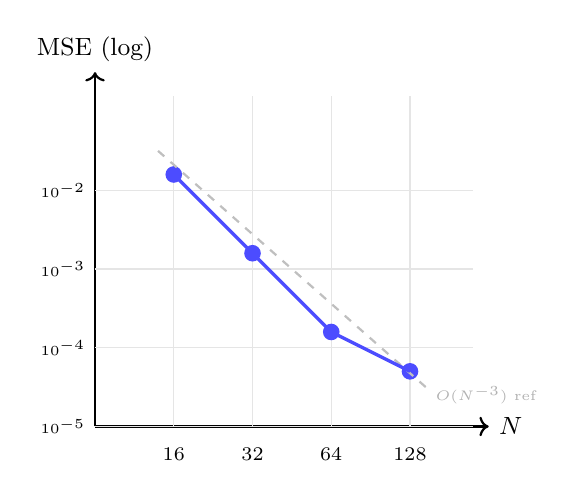
\begin{tikzpicture}[scale=1.0]
% Axes (log-log)
\draw[->, thick] (0,0) -- (5,0) node[right, font=\small]{$N$};
\draw[->, thick] (0,0) -- (0,4.5) node[above, font=\small]{MSE (log)};
% Grid
\foreach \x/\lbl in {1/16, 2/32, 3/64, 4/128} {
    \draw[gray!20] (\x,0) -- (\x,4.2);
    \node[below, font=\scriptsize] at (\x,-0.15) {\lbl};
}
\foreach \y/\lbl in {0/$10^{-5}$, 1/$10^{-4}$, 2/$10^{-3}$, 3/$10^{-2}$} {
    \draw[gray!20] (0,\y) -- (4.8,\y);
    \node[left, font=\tiny] at (0,\y) {\lbl};
}
% Data points (placeholder style)
\fill[blue!70] (1,3.2) circle (3pt);
\fill[blue!70] (2,2.2) circle (3pt);
\fill[blue!70] (3,1.2) circle (3pt);
\fill[blue!70] (4,0.7) circle (3pt);
% Reference line (3rd order)
\draw[gray!50, dashed, thick] (0.8,3.5) -- (4.2,0.5);
\node[gray!60, font=\tiny, anchor=west] at (4.2,0.4) {$O(N^{-3})$ ref};
% Connect points
\draw[very thick, blue!70] (1,3.2) -- (2,2.2) -- (3,1.2) -- (4,0.7);
\end{tikzpicture}
\end{column}

\begin{column}{0.42\textwidth}
\small
\textbf{Convergence data (experiments in progress):}

\vspace{0.2cm}
\begin{tabular}{cc}
$N$ & MSE \\
\midrule
16 & $\cdots$ \\
32 & $\cdots$ \\
64 & $\cdots$ \\
128 & $\cdots$ \\
\end{tabular}

\vspace{0.3cm}
\textbf{Expected behavior:}
\begin{itemize}
    \item Error decreases monotonically with $N$
    \item Effective $\sim 3$rd-order for $N{=}16{\to}64$
    \item Rigorous rate analysis deferred
\end{itemize}
\end{column}
\end{columns}
\end{frame}

% ---- Slide 16: Allen-Cahn ----
\begin{frame}{Allen--Cahn Benchmark}

\begin{columns}[T]
\begin{column}{0.6\textwidth}
\centering
\textbf{PDE:} $\partial_t u = \varepsilon^2\Delta u + u(1-u^2)$, \;$u\in[-1,1]$

\vspace{0.3cm}
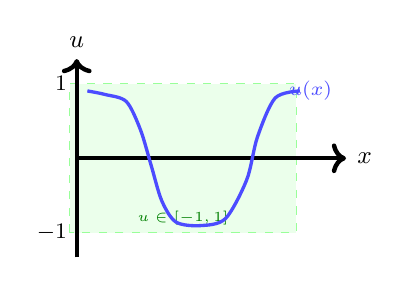
\begin{tikzpicture}[scale=0.9]
% Admissible region (drawn FIRST so axes are on top)
\fill[green!8] (-0.1,-1.05) rectangle (3.1,1.05);
\draw[green!40, dashed] (-0.1,-1.05) rectangle (3.1,1.05);
\node[green!50!black, font=\tiny] at (1.5,-0.85) {$u\in[-1,1]$};
% Axes (drawn AFTER green region so they are visible)
\draw[->, ultra thick] (0,0) -- (3.8,0) node[right, font=\small]{$x$};
\draw[->, ultra thick] (0,-1.4) -- (0,1.4) node[above, font=\small]{$u$};
% Tick labels
\node[left, font=\footnotesize] at (0,-1.05) {$-1$};
\node[left, font=\footnotesize] at (0,1.05) {$1$};
% Allen-Cahn phase-field: sharp interface between -1 and +1
\draw[very thick, blue!70, smooth] plot coordinates {
  (0.15,0.95) (0.4,0.9) (0.7,0.8) (0.9,0.4)
  (1.05,-0.1) (1.2,-0.6) (1.4,-0.9) (1.75,-0.95)
  (2.1,-0.85) (2.4,-0.3) (2.55,0.3) (2.8,0.85) (3.15,0.95)};
\node[blue!70, font=\scriptsize] at (3.3,0.95) {$u(x)$};
\end{tikzpicture}

\vspace{0.2cm}
\small
$\varepsilon=0.1$, $N=64$, $\Delta t=0.1$, $T_{\max}=2.0$
\end{column}

\begin{column}{0.37\textwidth}
\small
\textbf{Our guarantees (by construction):}

\vspace{0.2cm}
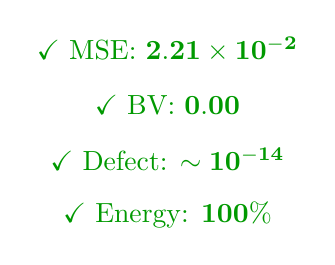
\begin{tikzpicture}[
    check/.style={green!60!black, font=\normalsize}
]
\node[check] at (0, 2.5) {$\checkmark$ MSE: $\mathbf{2.21\times10^{-2}}$};
\node[check] at (0, 1.8) {$\checkmark$ BV: $\mathbf{0.00}$};
\node[check] at (0, 1.1) {$\checkmark$ Defect: $\mathbf{\sim10^{-14}}$};
\node[check] at (0, 0.4) {$\checkmark$ Energy: $\mathbf{100\%}$};
\end{tikzpicture}

\vspace{0.3cm}
\textbf{vs.\ baselines} (experiments in progress):
\begin{itemize}
    \item FNO/ResNet: $\cdots$
\end{itemize}

\vspace{0.15cm}
\alert{Architectural guarantees transfer to Allen--Cahn.}
\end{column}
\end{columns}
\end{frame}

% ---- Slide 17: Burgers ----
\begin{frame}{Viscous Burgers Benchmark}

\begin{columns}[T]
\begin{column}{0.6\textwidth}
\centering
\textbf{PDE:} $\partial_t u + u\,\partial_x u = \nu\,\partial_{xx} u$, \;$u\in[-1,1]$

\vspace{0.3cm}
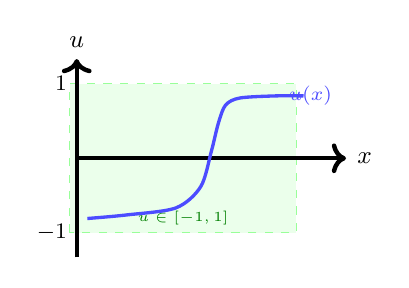
\begin{tikzpicture}[scale=0.9]
% Admissible region (drawn FIRST so axes are on top)
\fill[green!8] (-0.1,-1.05) rectangle (3.1,1.05);
\draw[green!40, dashed] (-0.1,-1.05) rectangle (3.1,1.05);
\node[green!50!black, font=\tiny] at (1.5,-0.85) {$u\in[-1,1]$};
% Axes (drawn AFTER green region so they are visible)
\draw[->, ultra thick] (0,0) -- (3.8,0) node[right, font=\small]{$x$};
\draw[->, ultra thick] (0,-1.4) -- (0,1.4) node[above, font=\small]{$u$};
% Tick labels
\node[left, font=\footnotesize] at (0,-1.05) {$-1$};
\node[left, font=\footnotesize] at (0,1.05) {$1$};
% Burgers viscous shock: smooth steep transition
\draw[very thick, blue!70, smooth] plot coordinates {
  (0.15,-0.85) (0.7,-0.8) (1.4,-0.7) (1.75,-0.4)
  (1.9,0.1) (2.0,0.5) (2.1,0.75) (2.3,0.85) (2.8,0.88) (3.2,0.88)};
\node[blue!70, font=\scriptsize] at (3.3,0.88) {$u(x)$};
\end{tikzpicture}

\vspace{0.2cm}
\small
$\nu=0.01$, $N=64$, $\Delta t=0.05$, $T_{\max}=1.0$
\end{column}

\begin{column}{0.37\textwidth}
\small
\textbf{Our guarantees (by construction):}

\vspace{0.2cm}
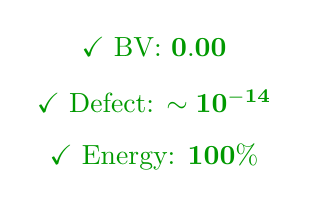
\begin{tikzpicture}[
    check/.style={green!60!black, font=\normalsize}
]
\node[check] at (0, 2.5) {$\checkmark$ BV: $\mathbf{0.00}$};
\node[check] at (0, 1.8) {$\checkmark$ Defect: $\mathbf{\sim10^{-14}}$};
\node[check] at (0, 1.1) {$\checkmark$ Energy: $\mathbf{100\%}$};
\end{tikzpicture}

\vspace{0.2cm}
\textbf{vs.\ baselines:}
\begin{itemize}
    \item FNO: BV $15.4\%$, defect $2.7\times10^{-4}$
    \item ResNet: BV $6.6\%$, defect $1.3\times10^{-3}$
\end{itemize}

\vspace{0.15cm}
\textbf{Note:} Burgers is \emph{non-gradient} --- expressivity guarantee does not formally apply, but architectural guarantees hold regardless.
\end{column}
\end{columns}
\end{frame}

% ---- Slide 18: Ablation ----
\begin{frame}{Ablation Study (Fisher--KPP)}

\begin{columns}[T]
\begin{column}{0.5\textwidth}
\centering
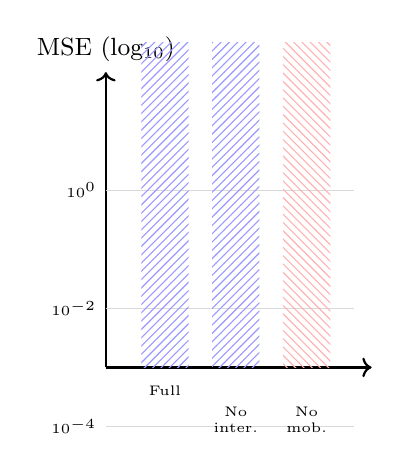
\begin{tikzpicture}[scale=0.75]
% Bar chart
\draw[->, thick] (0,0) -- (0,5) node[above, font=\small]{MSE (log$_{10}$)};
\draw[->, thick] (0,0) -- (4.5,0);
% Grid
\foreach \y/\lbl in {-4/$10^{-4}$, -2/$10^{-2}$, 0/$10^{0}$} {
    \draw[gray!30] (0, {\y+3}) -- (4.2, {\y+3});
    \node[left, font=\tiny] at (0, {\y+3}) {\lbl};
}
% Full
\fill[blue!60, pattern=north east lines, pattern color=blue!40] (0.6,0) rectangle (1.4, 5.5);
\node[below, font=\tiny] at (1.0, -0.15) {Full};
% No interaction
\fill[blue!60, pattern=north east lines, pattern color=blue!40] (1.8,0) rectangle (2.6, 5.5);
\node[below, font=\tiny, text width=1.2cm, align=center] at (2.2, -0.5) {No\\inter.};
% No mobility
\fill[red!50, pattern=north west lines, pattern color=red!30] (3.0,0) rectangle (3.8, 5.5);
\node[below, font=\tiny, text width=1.2cm, align=center] at (3.4, -0.5) {No\\mob.};
\end{tikzpicture}
\end{column}

\begin{column}{0.47\textwidth}
\small
\textbf{Findings (experiments in progress):}

\vspace{0.2cm}
\begin{itemize}
    \item Full \& No-interaction: comparable MSE (reaction term dominates Fisher--KPP)
    \item \textcolor{red!70}{No-mobility}: significantly worse --- $K_\theta(z)$ is the \textbf{critical component}
\end{itemize}

\vspace{0.2cm}
\textbf{All variants:} exact boundary compliance ($0.00$)

\vspace{0.15cm}
$\Rightarrow$ Architectural guarantee robust to component removal
\end{column}
\end{columns}
\end{frame}

% ---- Slide: Comparison with Classical Methods ----
\begin{frame}{Comparison with Classical Structure-Preserving Methods}

\begin{center}
\small
\begin{tabular}{lcc}
\toprule
\textbf{Method} & \textbf{Known $\cF$?} & \textbf{Guarantee} \\
\midrule
IRP schemes [Zhang \& Shu, 2010] & Yes & Invariant region \\
SSP integrators [Gottlieb, Shu \& Tadmor, 2001] & Yes & Convex constraints \\
Entropy-stable [Ju, Li \& Qiao, 2022] & Yes & Energy dissipation \\
\midrule
\textbf{Ours} & \textbf{No (learned)} & \textbf{All three by construction} \\
\bottomrule
\end{tabular}
\end{center}

\vspace{0.3cm}
\begin{itemize}
    \item Classical methods: design the \emph{scheme} for a known PDE
    \item Ours: constrain the \emph{learned vector field} itself
    \item Sigmoid map $\leftrightarrow$ positivity limiter; PSD mobility $\leftrightarrow$ dissipative integrator
    \item Key difference: we \emph{learn} the generator within a structurally constrained model class
\end{itemize}
\end{frame}

% ============================================================
\section{Conclusion}
% ============================================================

% ---- Slide 19: Summary ----
\begin{frame}{Summary and Take-Home Message}

\begin{columns}[T]
\begin{column}{0.5\textwidth}
\begin{block}{Core idea}
\centering
\small
\renewcommand{\arraystretch}{1.15}
\begin{tabular}{cl}
\toprule
\textbf{Design} & \textbf{Guarantee} \\
\midrule
sigmoid map $g$ & admissibility \\
$K\succ 0$ + gradient flow & dissipation \\
ODE flow & exact semigroup \\
\bottomrule
\end{tabular}
\end{block}

\vspace{0.15cm}
\begin{block}{Contributions}
\begin{enumerate}
    \item Semigroup-level error decomposition:\\
    $\|u^n - \cS_{n\Delta t}u_0\| \leq \varepsilon_{\mathrm{app}} + n\,\varepsilon_{\mathrm{sg}}$
    \item Architecture with $\varepsilon_{\mathrm{sg}}=0$ by construction
    \item Transfer theorem + universal approximation
\end{enumerate}
\end{block}
\end{column}

\begin{column}{0.47\textwidth}
\begin{alertblock}{Open Problems}
\begin{enumerate}
    \item Global flow existence for $\beta_V = 0$
    \item PDE-level transfer rigor
    \item Expressivity for non-gradient generators
    \item Extension to higher dimensions
\end{enumerate}
\end{alertblock}

\vspace{0.2cm}
\begin{beamercolorbox}[wd=\linewidth,rounded=true,shadow=true,sep=0.5em]{block title}
\centering
\large\textbf{Physics should be built into}\\[3pt]
\large\textbf{the architecture,}\\[3pt]
\large\textbf{not just the loss function.}
\end{beamercolorbox}

\vspace{0.2cm}
\centering
\small
{\color{gray} Three structural laws $\to$ three architectural constraints}\\[2pt]
{\color{gray} $\to$ guarantees hold for \emph{every} $\theta$, not just after training}
\end{column}
\end{columns}
\end{frame}

% ---- Thank You ----
\begin{frame}
\centering
\vspace{1.5cm}
{\Huge \textbf{Thank You}}\\[1cm]
{\Large Questions?}\\[1.5cm]
{\normalsize
Preprint available upon request\\[0.3cm]
}
\end{frame}

\end{document}
